\chapter{Intrabundle - An OSGi Bundle Introspection Tool}


\section{Introduction}
It was clear in previous chapters that modular and non modular applications have many differences and specific features hence the need for dedicated approach for quality analysis. This chapter presents a tool called \emph{Intrabundle} \citep{intrabundle github 2014}, an open source Java based application created in the context of this work. Intrabundle introspects OSGi projects collecting useful information and calculates OSGi bundle and project \textbf{internal quality}.  


\section{Design Decisions}
To analyze and extract data from large code bases of OSGi projects, which can vary from KLOCs to thousands of KLOCs, there was the need of a lightweight approach. Some \emph{functional requirements} were:

\begin{itemize}
\item Analyze different formats of OSGi projects like Maven\footnote{\href{http://maven.apache.org/index.html}{Maven} is a build tool for Java}, Eclipse projects and BND\footnote{\href{http://bndtools.org/}{BND} is a tool to easy OSGi projects development}; 
\item It should be able to dive deep into projects source code like counting methods calls, differentiate classes and interfaces and so on;  
\item Get general informations like project version, revision or latest commit in source repository;
\item Should be easy analyze lots of projects;
\item Should output a detailed Human readable quality report so the extracted information can be analyzed.
\end{itemize}

and the following \emph{non functional requirements}:

\begin{itemize}
\item Only open sourced projects\footnote{Projects that have its source code made available with a license in which the copyright holder provides the rights to study, change and distribute the software to anyone and for any purpose} because we focus on internal quality where the code is important;
\item The tool should be lightweight to analyze real, complex and huge OSGi projects;
\item Find and Introspect manifest files where valuable OSGi information rely; 
\item Should be testable;
\item Fast;
\item Use Java to leverage the author's experience in the language;
\item Use a good file system API\footnote{An API expresses a software component in terms of its operations, inputs, outputs, and underlying types.} because file manipulation is one of the most frequent tasks the tool should perform.\\*
\end{itemize}
 

The following alternatives were evaluated:

\begin{enumerate}
\item Build a standalone Java client application using javaFX\footnote{\href{http://docs.oracle.com/javase/8/javase-clienttechnologies.htm}{JavaFX} is a set of graphics and media packages that enables developers to design, create, test, debug, and deploy rich client applications};
\item Create an eclipse plugin\footnote{\href{https://wiki.eclipse.org/FAQ_What_is_a_plug-in\%3F}{Eclipse plug-ins} are software components with the objective to extend Eclipse IDE};
\item Create a  Maven plugin\footnote{Maven is a build tool that consists of a core engine which provides basic project-processing capabilities and build-process management, and a host of \emph{plugins} which are used to execute the actual build tasks.};
\item Build the tool on top of JBoss Forge;
\item Extend an existing static/internal analysis tool like PMD.
\end{enumerate}

The chosen among the above options was JBoss Forge, due to the following facts:

\begin{itemize}
\item Works inside and outside eclipse;
\item Works regardless of build tool;
\item As its a command line tool its very lightweight and can analyze multiple OSGi projects at the same time;
\item The programing model is based on top of the so called CDI\footnote{Context and Dependency Injection for the Java platform. CDI is a dependency injection framework where instead of dependencies construct themselves they are injected by some external means, in cae CDI} so managing Objects lifecycle and event is handled by CDI automatically;
\item Forge has a very well established and documented file system manipulation api based on java.io;
\item Forge is very flexible so generating quality reports is a matter of using a report API inside it;  
\item The author already had experience with JBoss Forge and CDI. 
\end{itemize}

Creating an eclipse plugin for analyzing OSGi projects could be not as lightweight as forge plugin. We would need eclipse started and OSGi projects imported inside IDE so the eclipse plugin could identify the project resources.

JavaFX would require use standard Java file system manipulation api(java.io) which has many caveats and pitfalls so for example its easy to create a memory leak or too many files opens error. Also with JavaFX there the need to implement the interface/GUI which is already well done in Eclipse or Forge.

Maven plugins are limited to maven projects.

PMD\footnote{A very nice tool for static code analysis. It is based on rules that can be created via xml or xpath expression. When a rule is violated it can output warns or errors to the console} has a very limited API so it could be hard to generate reports or analyze multiple projects using it. 


\section{Implementation Overview}

Intrabundle is composed by 3 Forge plugins, see section \ref{sec:forge:plugin} for details about Forge plugins. The first is \emph{BundlePlugin} which extracts OSGi bundle information, second is \emph{OSGiPlugin} that has a vision of all bundles composed by the project. Third is OSGiScan a plugin responsible for scanning OSGi bundles recursively in file system. Another component in the architecture is \emph{MetricsCalculator} that calculates bundle and OSGi project quality based on metrics produced by OSGiPlugin and BundlePlugin.

Intrabundle also provides 2 facets, see section \ref{sec:forge:facet} for details about Forge facets. \emph{BundleFacet} and \emph{OSGiFacet}, both restricts commands provided by BundlePlugin and OSGiPlugin in the context of OSGi bundle and project respectively. BundleFacet is active when user enter on a directory containing an OSGiBundle and OSGiFacet is active when user enters on a directory that contains at least one OSGiBundle. When BundleFacet is active then OSGiFacet is disabled meaning that only BundlePlugin commands will be active. 

Another important component in Intrabundle architecture is the Project Locator, see section \ref{sec:forge:locator} for details about Forge locators. Intrabundle provides 2 locators. The first is \emph{BundleLocator} that creates a Forge project object named \emph{OSGiModule} representing and gathering data related to OSGi bundle. BundleLocator is activated when user is at an OSGi bundle directory. The second is \emph{OSGiProjectLocator} which creates a Forge project object named \emph{OSGiProject} representing an OSGi project which is a collection of bundles. OSGiProject locator is activated when user is in a directory that has at least one child directory that is an OSGiBundle.          

Figure \ref{intrabundle-arch} illustrates Intrabundle architecture:

\begin{figure}[h]
\caption{Intrabundle Architecture}
\label{intrabundle-arch}
\centering
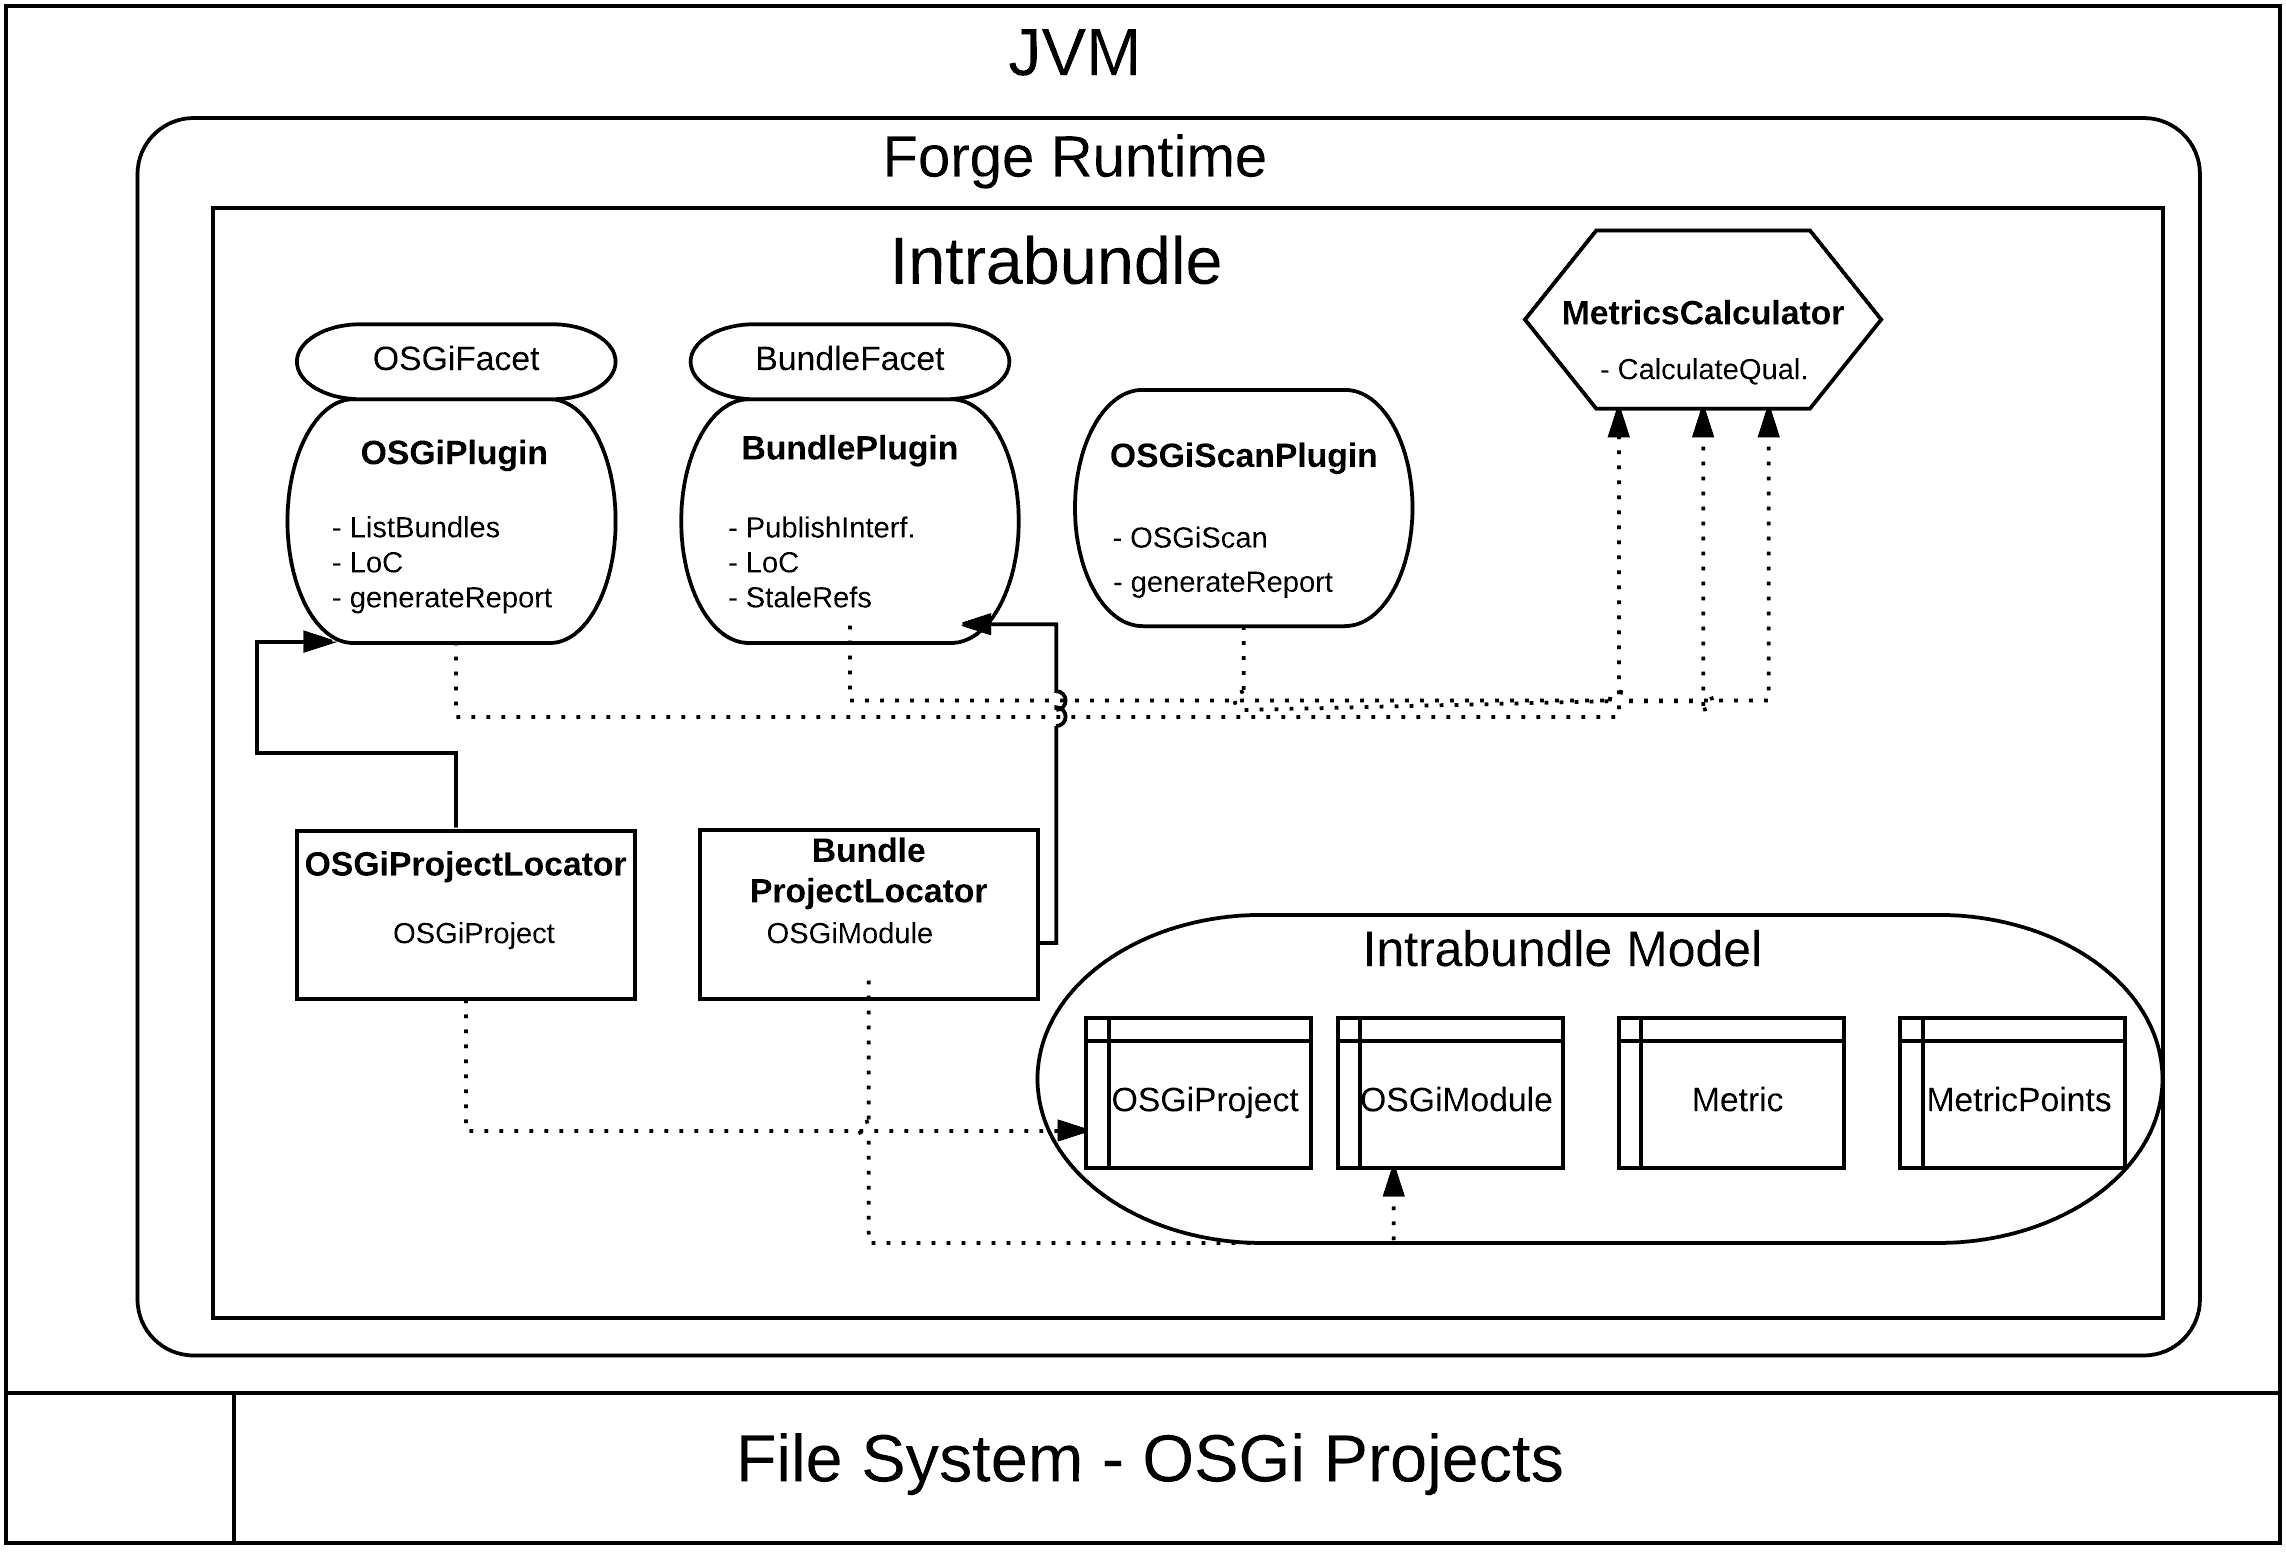
\includegraphics[scale=0.8]{intrabundle-arch}
\end{figure}  
\FloatBarrier


\section{Identifying OSGi Projects and Bundles}
One important task that both \emph{facets} and \emph{locators}, provided by Intrabundle, perform is identifying OSGi bundles or OSGi projects. To do that the tool searches for OSGi meta data in \emph{MANIFEST} file\footnote{The manifest is a special file that can contain information about the files packaged in a JAR file. By tailoring this "meta" information that the manifest contains, you enable the JAR file to serve a variety of purposes.}. So identifying bundles is as simple as locating the Manifest and verifies if it's content has OSGi information. The main problem is that the manifest location can vary depending on the project format. Table \ref{osgi-project-type} lists the types of OSGi projects Intrabundle recognizes:     

\begin{table}[h]
\caption{Supported types of OSGi projects}
\label{osgi-project-type}
\begin{center}
    \begin{tabular}{  p{4cm} | p{6cm} }
    \Xhline{2\arrayrulewidth}
    Type & Manifest location \\  \hline
    Maven projects & /src/main/resource/META-INF.\\ \hline
    Maven using BND tools & pom.xml\footnote{It's a xml configuration file responsible for project build life cycle and dependencies} with maven-bundle-plugin.\\ \hline
    Standard Eclipse Java projects & /META-INF\\ \hline
    Standard BND Tools & bnd.bnd file in any subfolder.\\ \hline
    Package based bundles(Jitsi project) & each package has a manifest.\\  
   \Xhline{2\arrayrulewidth}

    \end{tabular}
\end{center}
\end{table}
\FloatBarrier

In the extent of this work, \textbf{OSGi projects} are collections of OSGi bundles in the same directory but its also important to say that OSGi bundles can be installed from anywhere from the file system or network.

\section{Collecting Bundle Data}
After identifying OSGi bundles and OSGi projects Intrabundle needs to extract useful information from them. Table \ref{extracted-data} shows which information the tool is collecting:

\begin{table}[h]
\caption{Extracted data from OSGi projects}
\label{extracted-data}
\begin{center}
    \begin{tabular}{  p{4cm} | p{8cm} }
    \Xhline{2\arrayrulewidth}
    Name & Description\\  \hline
    Loc & Lines of code.\\ \hline
    Declarative services & Verifies if bundles uses declarative service\footnote{Is a component model that simplifies the creation of components that publish and/or reference OSGi Services.}.\\ \hline
    Ipojo & Verify if bundles uses Ipojo\footnote{Is a service component runtime aiming to simplify OSGi application development} \\ \hline
    Blueprint & Verify if bundles uses Blueprint\footnote{Is a way of instantiating and consuming services provided by others by means of an external XML configuration file} \\ \hline
    Stale References & Looks for possible Stale services references.\\ \hline
    Publishes Interface & Verifies if bundle exposes only its interfaces(API).\\ \hline
    Declares permission & Verifies if bundle declares permission.\\ \hline
    Number of classes & Counts bundle's classes.\\ \hline
    Number of abstract classes & Counts bundle's abstract classes.\\ \hline
    Number of interfaces & Counts bundle's interfaces.\\ \hline
    Bundle dependencies & Gather bundle dependencies.\\ \hline
    Required bundles & Gather bundle required bundles.\\ \Xhline{2\arrayrulewidth}
    \end{tabular}
\end{center}
\end{table}
\FloatBarrier 

Some observations about collected data. \textbf{Lines of code} are an indicative of high or low cohesion, if the component has too much lines of code its an evidence that it is probably doing more work then it should. LoC is a classical software metric that was adapted in this work to OSGi Bundles. 
\textbf{IPojo}, \textbf{Blueprint} and \textbf{Declarative Services} are recommended for managing OSGi services because they hide the "dirty work" of publishing and consuming services which sometimes may lead to incorrect behavior. For example forgetting to release a service when bundle is stopped.  
\textbf{Stale Services References}\footnote{Refers to code that may retain OSGi service references even when the providing bundles are gone \citep{Gama 2012}} are detected via approximation, in other words, Intrabundle counts the number of services \emph{gets} and \emph{ungets}\footnote{Operations that consume and release a service reference respectively} for each class a bundle has. If the number of gets and ungets are equal then the class have no stale references, otherwise it is considered as having stale references.
\textbf{Bundle dependencies} are calculated by looking at OSGi Manifest file in exported and imported packages. If bundle A \emph{imports} package \emph{x.y.z} and bundle B \emph{exports} package \emph{x.y.z} we say that bundle A depends on bundle B. 
\textbf{Required bundles} just counts the number of required bundles declared in manifest.
\textbf{Publishes interfaces} looks at bundle exported packages, if all exported packages contains only interfaces we say that bundle only imports interfaces.
\textbf{Declares permission} verifies if bundle implements security by contract searching for \emph{permission.perm} file.

Each information retrieved by Intrabundle is usually mapped to a Forge command, see Listing \ref{forge_command_example} which is the command that prints bundle exported packages to the Forge console:
\pagebreak
\begin{lstlisting}[language=java,label=forge_command_example,caption=Exported packages command]
 @Command(value = "exportedPackages",help = "list bundle exported packages")
 public void exportedPackages(PipeOut out){
      if(bundle.getExportedPackages().isEmpty()){
            out.println(messageProvider.getMessage("module.noExportedPackages"));
        }
      else{
          for (String s : bundle.getExportedPackages()) {
               out.println(s);
           }
       }
    }
\end{lstlisting}
\FloatBarrier

All the logic is inside \textbf{bundle} variable, which is an immutable object\footnote{Is an object whose state cannot be modified after it is created. A good practice and core principle in domain driven design \citep{Evans 2003}}, in method \emph{getExportedPackages}. The bundle variable is provided by a Forge locator when user navigates to a directory which is an OSGi bundle, as explained in section \ref{sec:forge:locator}. 

\section{Quality Calculation}
The data collected earlier will be materialized into six metrics that will be used to calculate OSGi projects quality. We saw on section \ref{sec:soft_metrics} that a software metric is a quantitative calculation of a software attribute. This section shows which metrics were created based on extracted information.


\subsection{Quality labels}
Every created metric in this work can be classified into the following \emph{quality labels}:

\begin{enumerate}
\item \textbf{STATE OF ART}: Metric fully satisfies good practices;
\item \textbf{VERY GOOD}: Satisfies most recommendations;
\item \textbf{GOOD}: Satisfies recommendations;
\item \textbf{REGULAR}: Satisfies some recommendations;
\item \textbf{ANTI PATTERN}: Does not satisfies any recommendation and follows some bad practices.
\end{enumerate}


\subsection{Metrics Created}

The first metric created is \textbf{LoC}, its the simplest one. LoC is based on bundle lines of code(excluding comments) meaning that the less lines of code more \emph{cohesion} the bundle has and easier to maintain it should be. This metric is an estimation, there is no exact LoC number because it depends on the context(e.g. complexity). To classify LoC metric we use the following rule:\newline


\(\text{LoC}=\begin{cases}
\text{STATE OF ART}& \text{if LoC <= 700},\\
\text{VERY GOOD}& \text{if LoC <= 1000}, \\
\text{GOOD}& \text{if LoC <= 1500}, \\
\text{REGULAR}& \text{if LoC <= 2000}, \\
\text{ANTI PATTERN}& \text{if LoC > 2000}. \\
\end{cases} \)\newline  

Second metric is \textbf{Publishes interfaces} meaning that bundles should hide their implementation and expose only it's API. It is a good practice expose only the API and hide the implementation details from consumers. This is considered an \emph{Usability pattern} \citep{Knoernschild 2012}. Here is how this metric is calculated:\newline

\(\text{Publishes interfaces}=\begin{cases}
\text{STATE OF ART}& \text{if publishes only interfaces},\\
\text{REGULAR}& \text{if not publishes only interfaces}, \\
\end{cases} \)  \newline

Next metric is \textbf{Bundle dependencies}, it evaluates the coupling between bundles. The less coupled a bundle is the more reusable and maintainable it will be. It is considered a base pattern called \emph{Manage Relationships} in \citep{Knoernschild 2012}. Here is how this metric is calculated by Intrabundle:\newline


\(\text{Bundle dependencies}=\begin{cases}
\text{STATE OF ART}& \text{if Bundle dependencies = 0},\\
\text{VERY GOOD}& \text{if Bundle dependencies <= 3}, \\
\text{GOOD}& \text{if Bundle dependencies <= 5}, \\
\text{REGULAR}& \text{if Bundle dependencies <= 9}, \\
\text{ANTI PATTERN}& \text{if Bundle dependencies >= 10}. \\
\end{cases} \)\newline 

Next one is \textbf{Uses framework}, in complex application it is important to usa a framework to manage bundle services. This metrics takes into account 3 well known frameworks by OSGi application: \emph{IPojo}, \emph{Declarative services} and \emph{Blueprint}: \newline

\(\text{Uses framework}=\begin{cases}
\text{STATE OF ART}& \text{if uses framework},\\
\text{REGULAR}& \text{if not using framework}, \\
\end{cases} \)  \newline

Next metric is \textbf{Stale references}, it focus on a very common problem in OSGi which can lead to resource and memory leaks \citep{Gama 2011}. Intrabundle calculate this metric by counting specific methods calls to OSGi services in a bundle. What Intrabundle does is an approximation and may lead to false positives. To get a real value for this software attribute one have to calculate it by dynamic analysis like done in \citep{Gama 2012}:\newline

\(NC = \sum_{i=1}^{n} \) where \textbf{n} = number of classes a bundle have. \newline
\(NS = \sum_{i=1}^{n} \) where \textbf{n} = number of stale references found. \newline

\(\text{Stale references}=\begin{cases}
\text{STATE OF ART}& \text{no stale references},\\
\text{GOOD}& \frac{NS}{NC} < 0.1, \\
\text{GOOD}& \frac{NS}{NC} < 0.25, \\
\text{REGULAR}& \frac{NS}{NC} < 0.5, \\
\text{ANTI PATTERN}& \frac{NS}{NC} >= 0.5. \\
\end{cases} \)\newline     

In other words if no stale references is found then this metric receives a \emph{state of art} quality label, if less then 10\% of bundle classes have stale references(number of get and unget doesn't match) then it receives \emph{very good} quality label, if > 10\% and < 25\% then it is \emph{good}, if the number of stale references is between 25\% and 50\% its is \emph{regular} but if it has 50\% or more classes with stale references then its considered an \emph{anti pattern}. 

The last metric created in this work is \textbf{Declares permission}, it is concerned with security. In this metric Intrabundle searches for permissions.perm file in the bundle, if it finds it then the metric is considered state of art: \newline


\(\text{Declares permission}=\begin{cases}
\text{STATE OF ART}& \text{if declares permission},\\
\text{REGULAR}& \text{if not declares permission}, \\
\end{cases} \)  \newline

\subsection{Quality Formula}

OSGi \emph{project} quality and \emph{bundle} quality are calculated by Intrabundle using the quality labels. Each quality \emph{label} adds points to bundle and project final quality which is based on percentage of quality points(QP) obtained. \emph{State of art} add \textbf{5QP}, \emph{Very good} \textbf{4QP}, \emph{Good} adds \textbf{3QP}, \emph{Regular} \textbf{2QP} and \emph{Anti pattern} adds \textbf{1QP}

\subsubsection{Bundle Quality}
Bundle final quality is calculated as a function of \emph{Total Quality Points} \textbf{TQP}, which is the total points obtained on each created metric, and \emph{Maximum Quality Points} \textbf{MQP}, the maximum points a bundle can have. MQP is equal to all metrics classified as State of art. Here is the formula:\newline    

\(MQP = \sum_{i=1}^{n} 5 \) where \textbf{n} = number of metrics. \newline

\(TQP = \sum_{i=1}^{n} q(i) \) where \textbf{n} = number of metrics and \textbf{q(i)} is QP obtained in metric \textbf{i}. \newline

 
\(
f(q) = \frac{TQP}{MQP};
\)
\newline
\newline
 if \( 1 <= f(q) > 0.9 \) then State of Art; \\*
 if \( 0.9 <= f(q) > 0.75 \) then Very Good; \\*
 if \( 0.75 <= f(q) > 0.6 \) then Good; \\*
 if \( 0.6 <= f(q) > 0.4 \) Regular; \\*
 if \( 0.4 <= f(q) \) then Anti Pattern;\\*

In terms of percentage of points obtained, more than 90\% of TQP is considered State of Art, between 90\% and 75\% is Very good quality, from 60\% to 75\% is Good, 40\% to 60\% is Regular and less than 40\% of TQP a bundle is considered Anti pattern in terms of software quality. 

For example imagine we have three metrics and a bundle has 5QP(State of art) and 3QP(Good quality label) in the other two metrics> In this case the MQP is 15 (5*3) and TQP is 11(5 + 3 +3). In this example the bundle quality is 11/15(73\%) which maps to \emph{Good} quality label. 


\subsubsection{Project Quality}
\label{sec:project-quality}
In Intrabundle, the quality of an OSGi project uses the same formula of bundle quality. The only difference is in MQP and TQP which in this case are based on bundles quality instead of metrics. In project quality the maximum point is calculated considering all bundle's quality as State of art, so for example if we have 3 bundles the MQP will be 15. TQP is just the sum of all bundles quality, here is the formula Intrabundle uses for \emph{project quality}:

\(MQP = \sum_{i=1}^{n} 5 \) where \textbf{n} = number of bundles in the project. \newline

\(TQP = \sum_{i=1}^{n} q(i) \) where \textbf{n} = number of bundles and \textbf{q(i)} is QP obtained by bundle \textbf{i}. \newline

 
\(
f(q) = \frac{TQP}{MQP};
\)
\newline
\newline
 if \( 1 <= f(q) > 0.9 \) then State of Art; \\*
 if \( 0.9 <= f(q) > 0.75 \) then Very Good; \\*
 if \( 0.75 <= f(q) > 0.6 \) then Good; \\*
 if \( 0.6 <= f(q) > 0.4 \) Regular; \\*
 if \( 0.4 <= f(q) \) then Anti Pattern;\\*

In terms of percentage it's also the same rule used for bundle's quality. For example if a project has 3 bundles, one has 5QP(State of art) and other two has 3QP(good) then MQP for this case is 15(5*3) and TQP is 11(5 + 3 +3). In this example project final quality is 11/15(73\%) which maps to \emph{Good} quality label. 

\subsubsection{Project metric quality}
\label{sec:project-quality-metric}
The last way to measure quality using Intrabundle is to analyze the project quality on each metric. The project quality in a metric is the sum of all \emph{bundles qualities} on that metric. The total points a bundle can have in a metric is considering all bundles State of art on that metric. The quality label for a project metric quality is also define as percentage of points obtained from maximum points:

\(MQP = \sum_{i=1}^{n} 5 \) where \textbf{n} = number of bundles in the project. \newline

\(TQP = \sum_{i=1}^{n} q(i) \) where \textbf{n} = number of bundles and \textbf{q(i)} is QP obtained by bundle \textbf{i} in the metric. \newline

 
\(
f(q) = \frac{TQP}{MQP};
\)
\newline
\newline
 if \( 1 <= f(q) > 0.9 \) then State of Art; \\*
 if \( 0.9 <= f(q) > 0.75 \) then Very Good; \\*
 if \( 0.75 <= f(q) > 0.6 \) then Good; \\*
 if \( 0.6 <= f(q) > 0.4 \) Regular; \\*
 if \( 0.4 <= f(q) \) then Anti Pattern;\\*

So for example if a project has 3 bundles, one has 5QP(State of art) in LoC and other two has 3QP(good) then MQP is 15(5*3) and TQP is 11(5 + 3 +3). In this example project final quality on LoC is 11/15(73\%) which maps to \emph{Good} quality label.  

\section{Intrabundle Reports}
\label{sec:intrabundle-reports}
The tool generates two reports based on information it collects from bundles so the it can be analyzed carefully in one place. The reports can be generated in various formats (txt, pdf, html, csv and excel). Figure \ref{intrabundle-report1} shows an example report:  

\begin{figure}[h]
\caption{Intrabundle general report}
\label{intrabundle-report1}
\centering
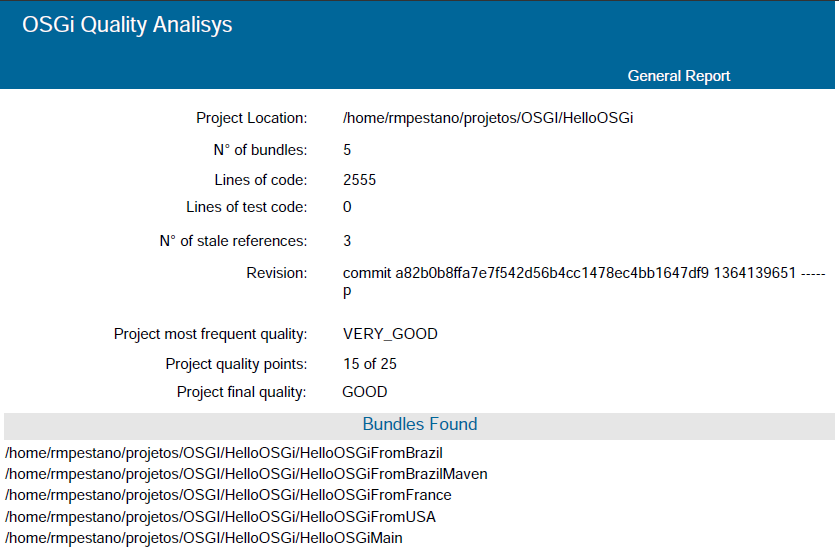
\includegraphics[scale=0.5]{intrabundle-report}
\end{figure}  
\FloatBarrier

The first section of the report gives an overall idea of the project, second part lists information of each bundles, see Figure \ref{intrabundle-report2} 

\begin{figure}[h]
\caption{Intrabundle general report - detailed section }
\label{intrabundle-report2}
\centering
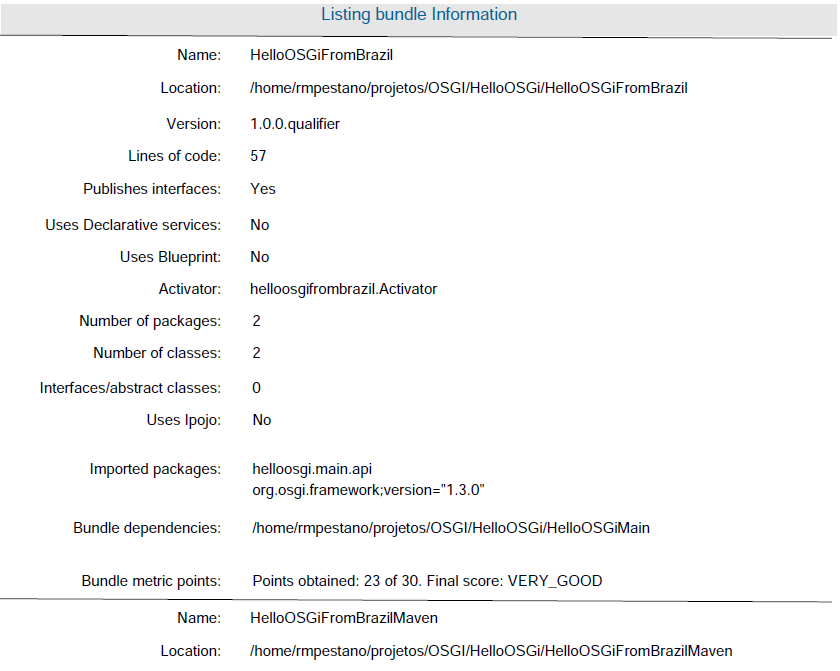
\includegraphics[scale=0.5]{intrabundle-report2}
\end{figure}  
\FloatBarrier

Another report Intrabundle generates is a metric report that details the punctuation of each metric, see Figure \ref{intrabundle-metrics-report}:  

\begin{figure}[h]
\caption{Intrabundle metrics report}
\label{intrabundle-metrics-report}
\centering
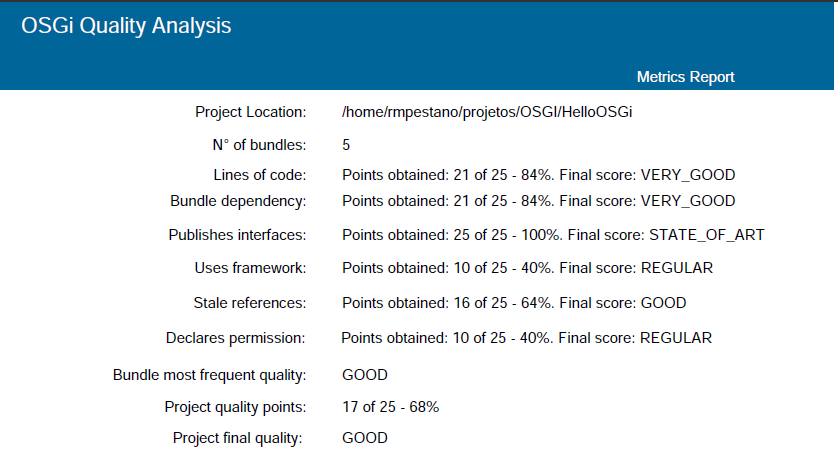
\includegraphics[scale=0.5]{intrabundle-metrics-report}
\end{figure}  
\FloatBarrier

As in general report, in metrics report the first section of the report gives an overall idea of the project, second part lists information of each bundles, see Figure \ref{intrabundle-metrics-report2} 

\begin{figure}[h]
\caption{Intrabundle metrics report - detailed section}
\label{intrabundle-metrics-report2}
\centering
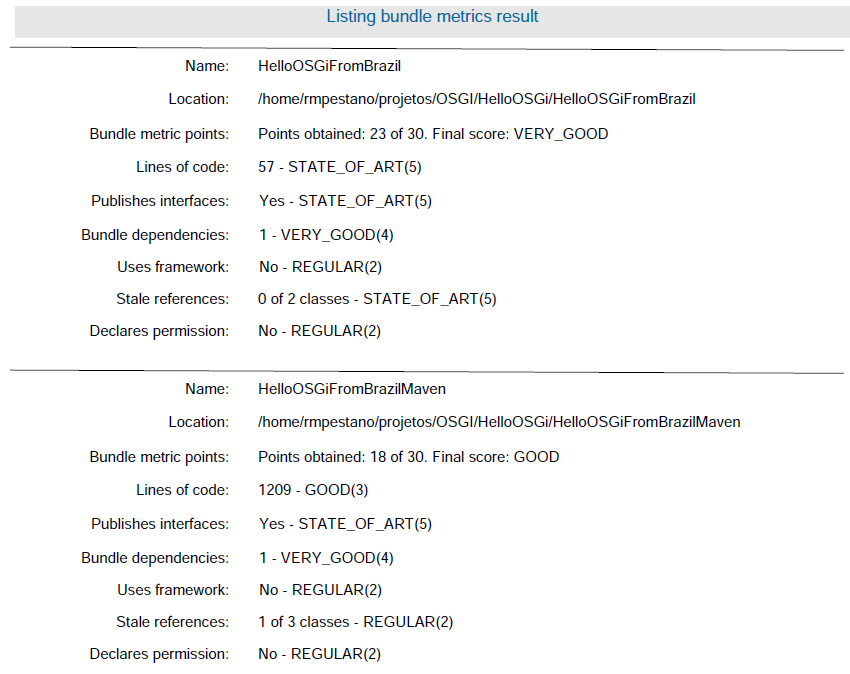
\includegraphics[scale=0.5]{intrabundle-metrics-report2}
\end{figure}  
\FloatBarrier

All reports generated by Intrabundle can be found online \cite{intrabundle reports 2014}.

\section{Intrabundle Quality}
In this section we will see how Intrabundle's quality is managed and how some concepts of \textit{section \ref{sec:quality}} were applied to the project. As the project is not OSGi based we can't apply Intrabundle's metrics on itself so we used classical approaches to assure the quality of the project.

\subsection{Internal quality}
Intrabundle internal quality is managed by PMD and JaCoCo. PMD is an static analysis tool and JaCoCo a dynamic analysis one. Both were presented in section \ref{ch2:qatools} with the objective to guarantee non functional requirements.

\subsubsection{Example}
 PMD was already illustrated at Chapter 2 as an example of static analysis tool. JaCoCo is used to calculate code coverage to track files and methods that automated tests are covering. Figure \ref{intrabundle-code-cover} shows JaCoCo code coverage report for Intrabundle:

\begin{figure}[h]
\caption{Intrabundle code coverage}
\label{intrabundle-code-cover}
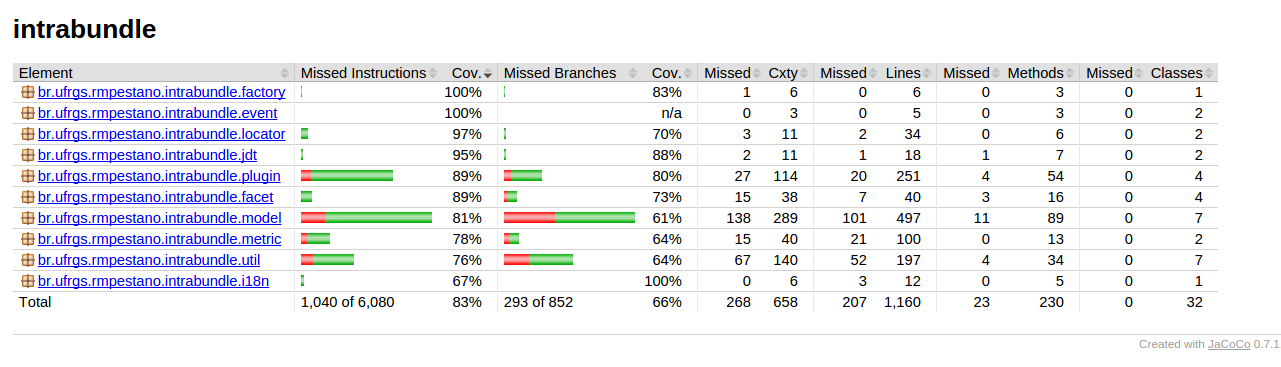
\includegraphics[scale=0.5]{intrabundle-code-coverage}
\end{figure}

\FloatBarrier

\subsection{External quality}
Intrabunde external quality is assured by automated whitebox tests so we can verify if Intrabundle is working as expected, if it meets its functional requirements.

\subsubsection{Example}
As of November 2014 Intrabundle performs 65 \textbf{integration tests} which can be defined as automated tests aimed to detect any inconsistencies between the software units that are integrated together. In this kind of automated tests the system must be running and in case of Intrabundle we also need the Forge runtime up and running during tests and that is done by Arquillian \citep{dan 2011}, an integration test platform. Figure \ref{intrabundle-integ-tests} shows the result of integration tests execution:

\begin{figure}[h]
\caption{Intrabundle integration tests}
\label{intrabundle-integ-tests}
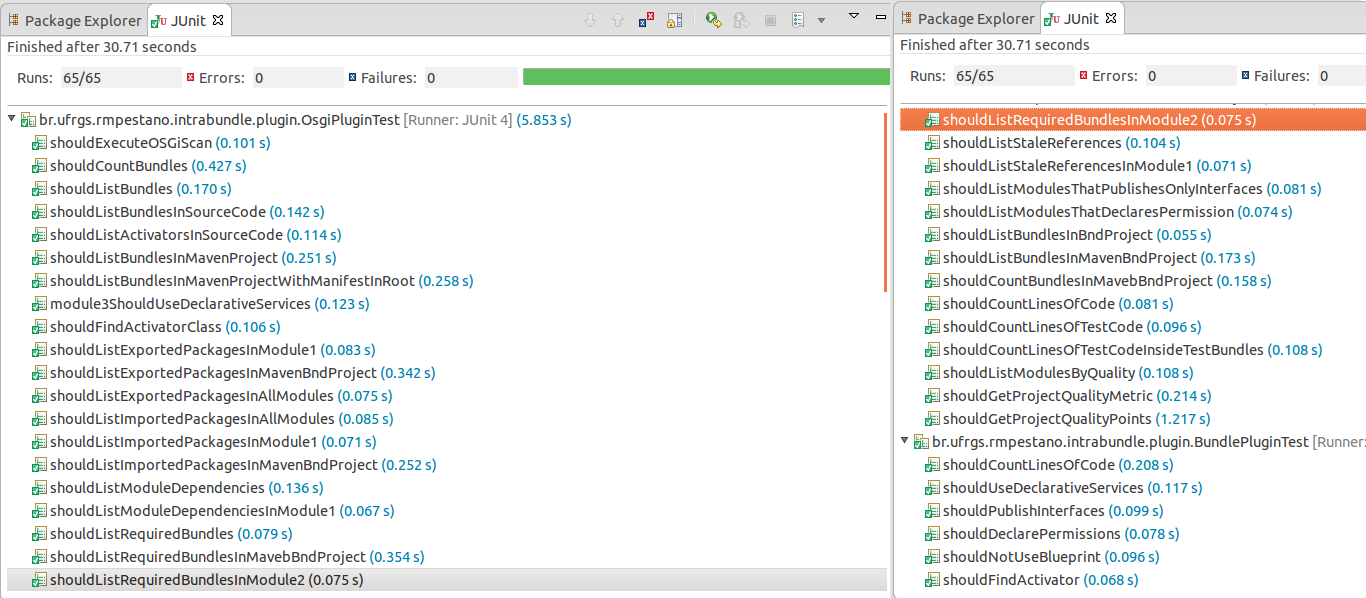
\includegraphics[scale=0.6]{intrabundle-external-quality}
\centering
\end{figure}

\FloatBarrier